\chapter{System Design and Methodology}
\label{Systemdesign}
The purpose of the design phase is to plan a solution to the problem specified by the requirement specification. This phase is the first step in moving from the problem domain to the solution domain. In other words, starting with what is needed, design takes us toward how to satisfy the needs. The design of a system is the most critical factor affecting
the quality of the software and it has a major impact on the latter phases, particularly testing and maintenance . Once the design phase is completed, we get a document with a plan for the solution which is used in implementation, testing and maintenance. The design activity is divided into two separate phases namely:
\begin{itemize}
    \item System Design
    \item Detailed Design
\end{itemize}
\section{System Design}
System Design aims to identify the modules that should be present in the system, the specification of these modules and how they interact with each other to produce the desired results. At the end of the system design, all the major data structures, file formats, output formats and major modules in the system and their specifications are decided.
The requirements obtained in earlier stages of the software development life cycle (SDLC) are translated into a thorough blueprint for creating the program during the phase known as system design. The architecture, parts, interfaces, and data structures must all be specified, together with the algorithms and functionalities they support. Software’s scalability, maintainability, and compliance with the requirements are all ensured through system design.
\newpage
\subsection{Data Flow Diagrams}
\subsubsection{Level 0 Data Flow}
The Level 0 Data Flow Diagram represents the FastTrack System's high-level interactions with its key users: Admin, Company, Delivery Personnel and Guests. Each entity exchanges information with the system, such as registration, authentication, package assignments and route details. This diagram provides an overview of data flow without detailing internal processes.
\begin{figure}[H]  % Use [H] to keep it under the correct title
\centering
    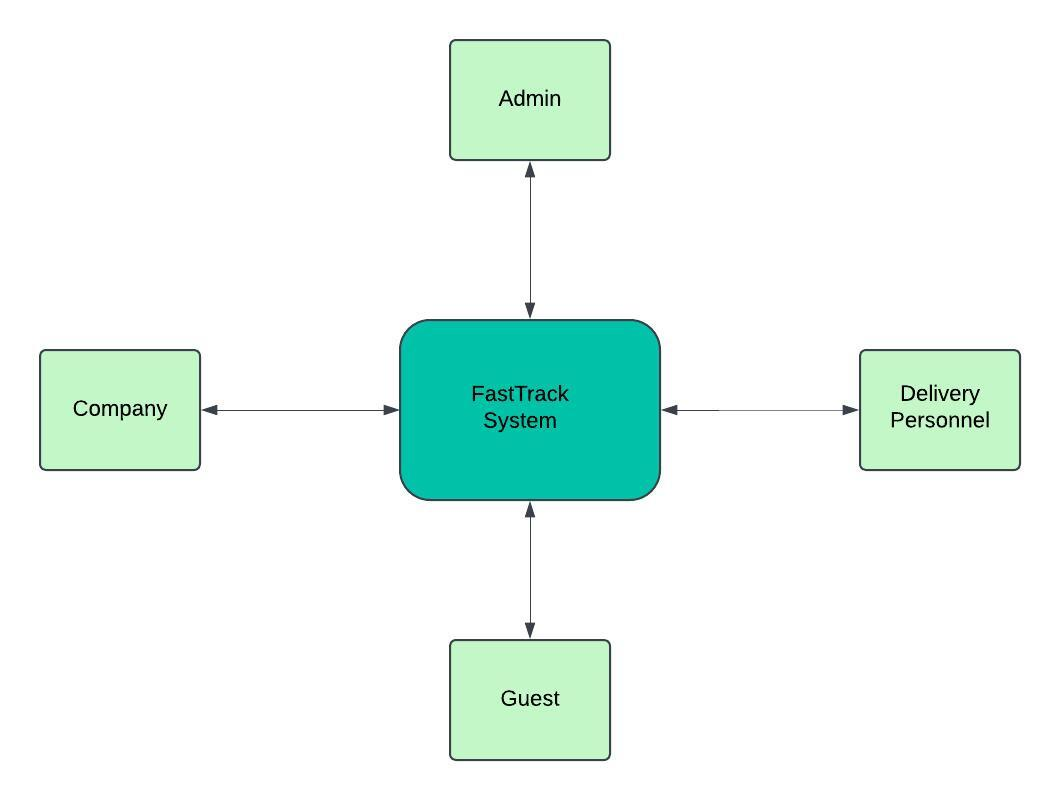
\includegraphics[scale=0.7]{Level 0 Data Flow.jpeg}
    \caption{Level 0 Data Flow}
    \label{fig:level0_data_flow}  % Fix label format (avoid spaces)
\end{figure}
\newpage
\subsubsection{Level 1 Data Flow}
The Level 1 Data Flow Diagram provides a detailed breakdown of the FastTrack System's interactions. It illustrates how different entities (Admin, Company, Delivery Personnel) provide data inputs like registration, package details, and updates, which are processed and stored in the system. The system interacts with data stores for Company Information, Delivery Personnel Data, and Package Details while ensuring smooth validation, updates, and retrieval of necessary information.
\begin{figure}[H]  % Use [H] to keep it under the correct title
\centering
    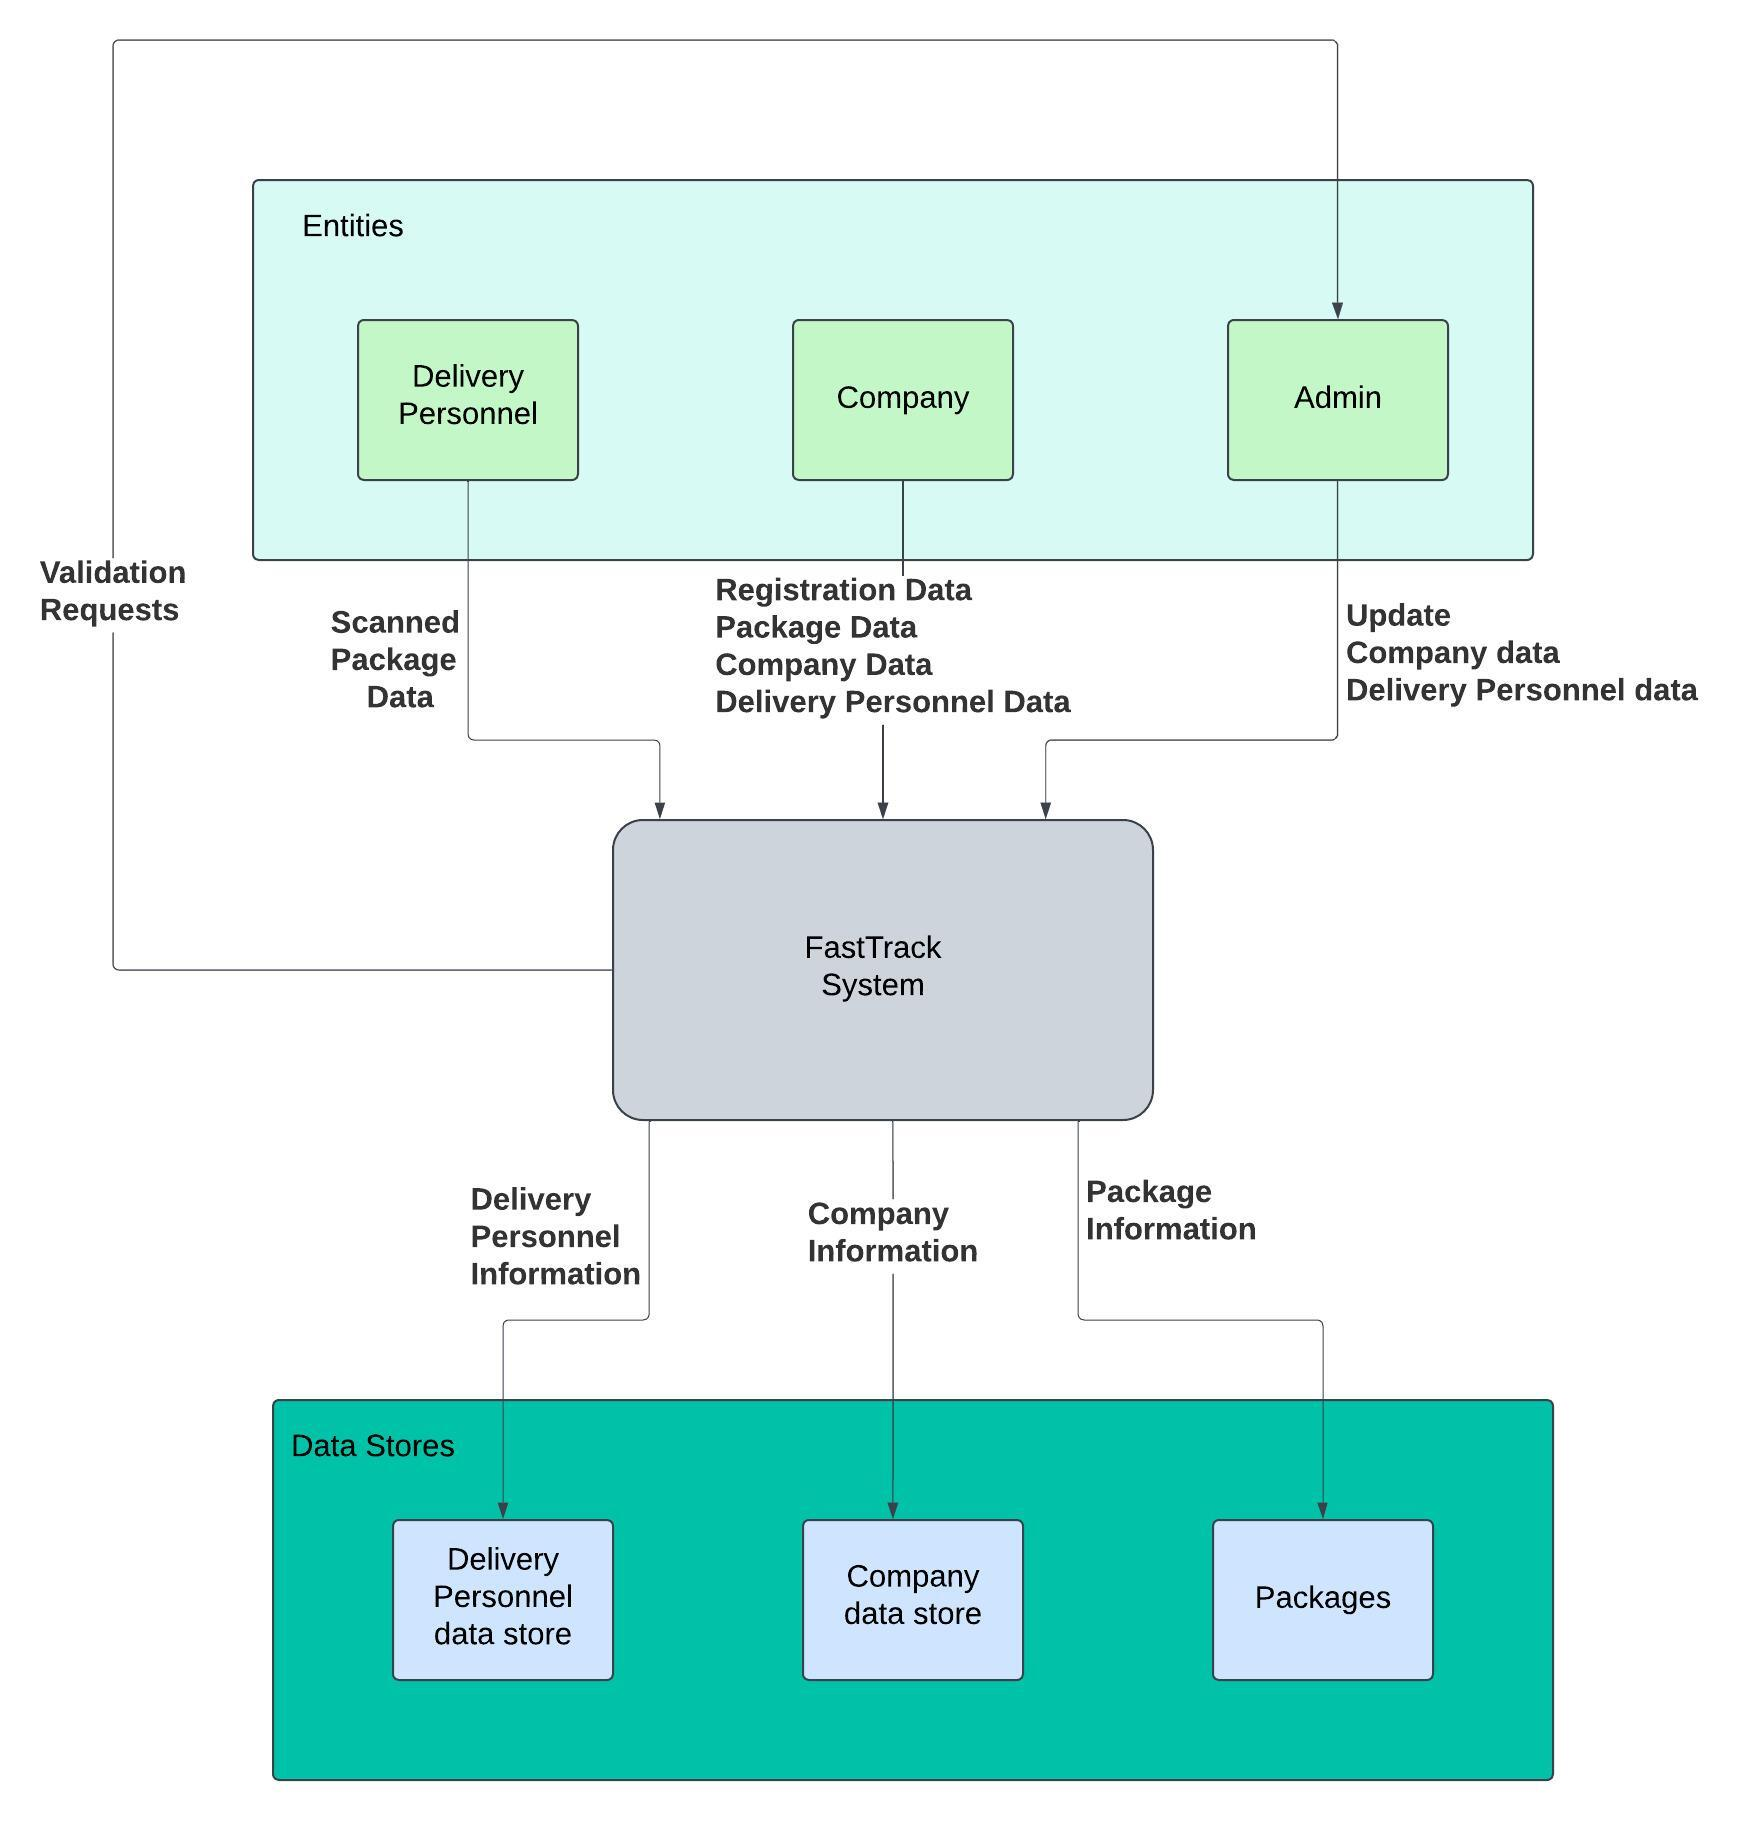
\includegraphics[scale=0.5]{Level 1 Data Flow.jpeg}
    \caption{Level 1 Data Flow}
    \label{fig:level1_data_flow}  % Fix label format (avoid spaces)
\end{figure}
\newpage
\subsection{Use Case Diagram}
The Use Case Diagram for the FastTrack illustrates how different users interact with the system’s functionalities. The main actors are Company, Delivery Personnel, Admin and Guest.
Company can register, arrange packages and generate optimized routes. Delivery Personnel can log in, scan packages, view package details and check optimized routes. Admin is responsible for validating registrations, granting login credentials and updating system information. Guests have limited access, such as browsing the map without logging in.
% \textbf{Actors \& Their Use Cases}
% \begin{enumerate}
%     \item Delivery Personnel 
%     \begin{itemize}
%         \item Login - Logs in using their credentials to manage the system.
%         \item Scan Package - Scans the package details before delivery.
%         \item Package Info - Views package details such as weight, size, and location.
%         \item Optimized Route Info - Gets the best route for deliveries.
%     \end{itemize}
%     \item Company
%     \begin{itemize}
%         \item Register - Registers itself on the platform.
%         \item Login - Logs in using their credentials to manage the system.
%         \item Arrange Packages - Organizes and assigns packages to delivery personnel.
%         \item Generate Optimized Route - Computes the best delivery route for efficiency.
%     \end{itemize}
%     \item Admin
%     \begin{itemize}
%         \item Login - Logs in using their credentials to manage the system.
%         \item Validate Registration - Approves new company registrations.
%         \item Grant Login ID - Provides login credentials to verified companies and personnel.
%         \item Update Info - Updates company and personnel information in the system.
%     \end{itemize}
%     \item Guest
%     \begin{itemize}
%         \item Browse Map - Views the map without logging in.
%     \end{itemize}
% \end{enumerate}

\begin{figure}[H]  % Use [H] to force the position
\centering
    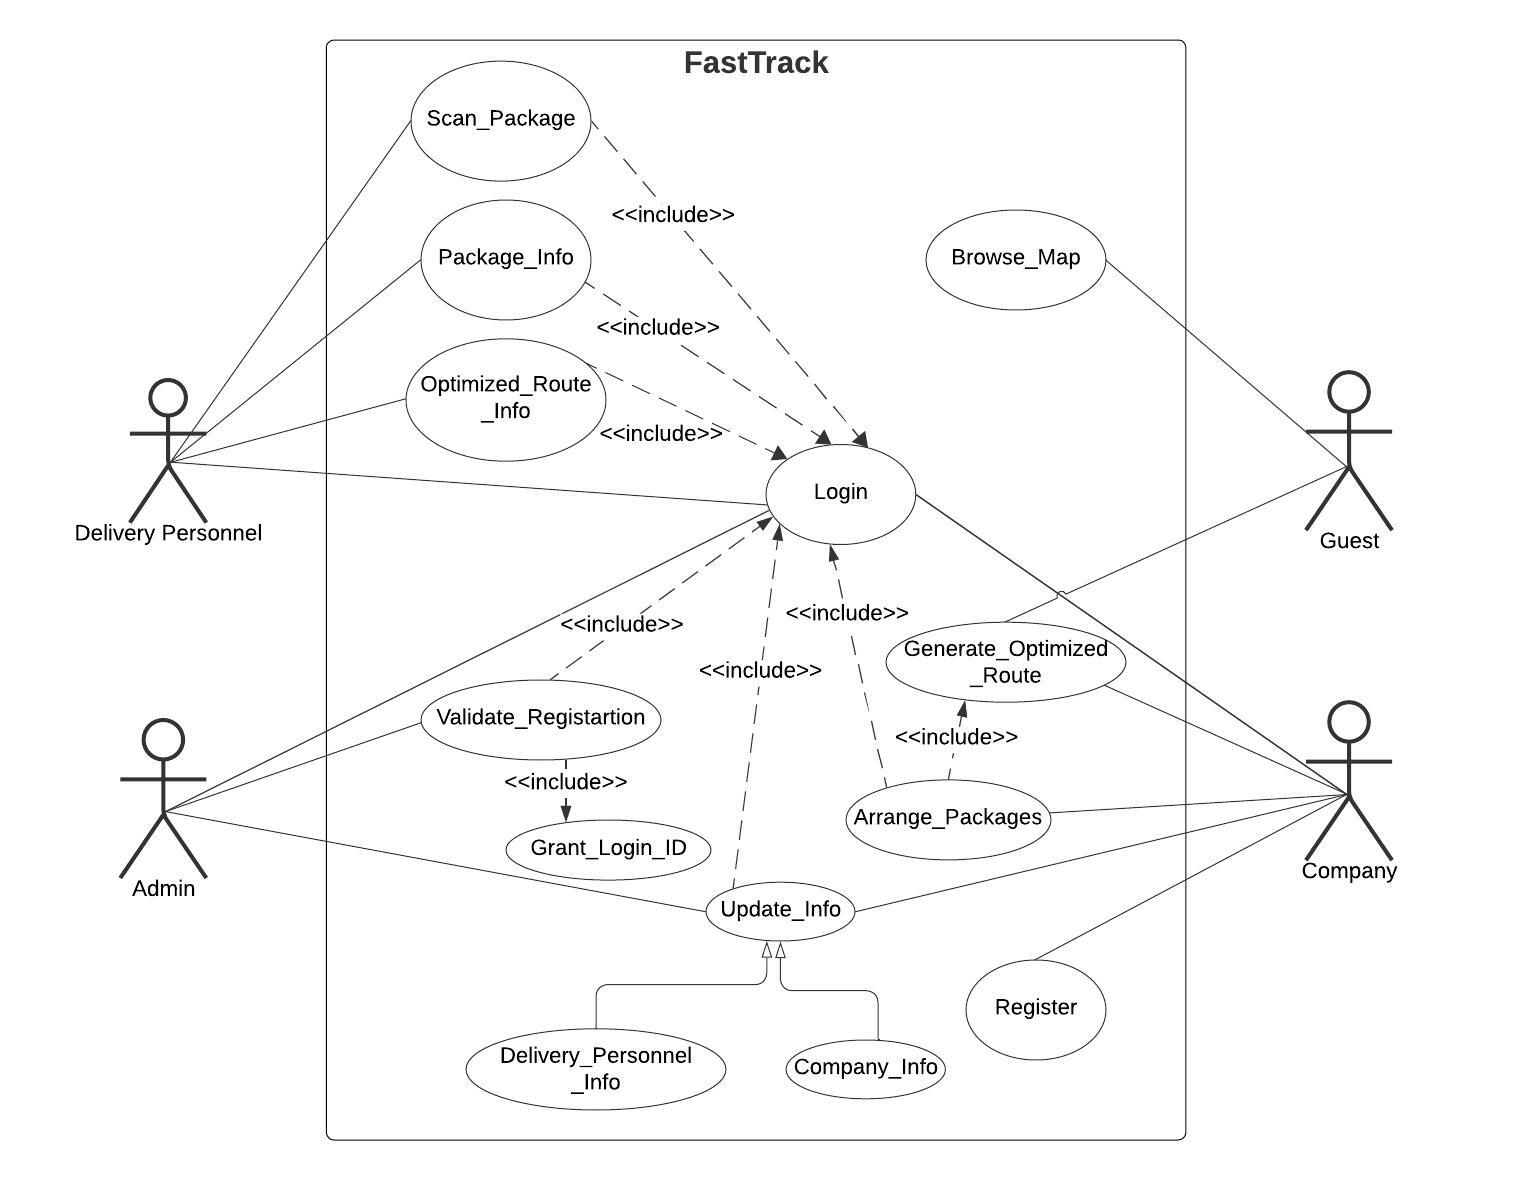
\includegraphics[scale=0.6]{Use case diagram (3).jpeg}
    \caption{Use Case Diagram}
    \label{fig:use_case}
\end{figure}
\newpage
\subsection{System Architecture Diagram}
The System Architecture of Fasttrack consists of a website, a Flutter mobile app, a Firebase database and integration with Google Maps API. The website allows companies to upload package details and assign delivery personnel, while the Flutter app enables delivery personnel to scan packages, receive optimized routes and update their delivery status in real time. Firebase acts as the central database, syncing data between the website and the app. The system also leverages Google Maps API for route optimization and navigation, ensuring efficient deliveries.
\begin{figure}[H]  % Use [H] to force the position
\centering
    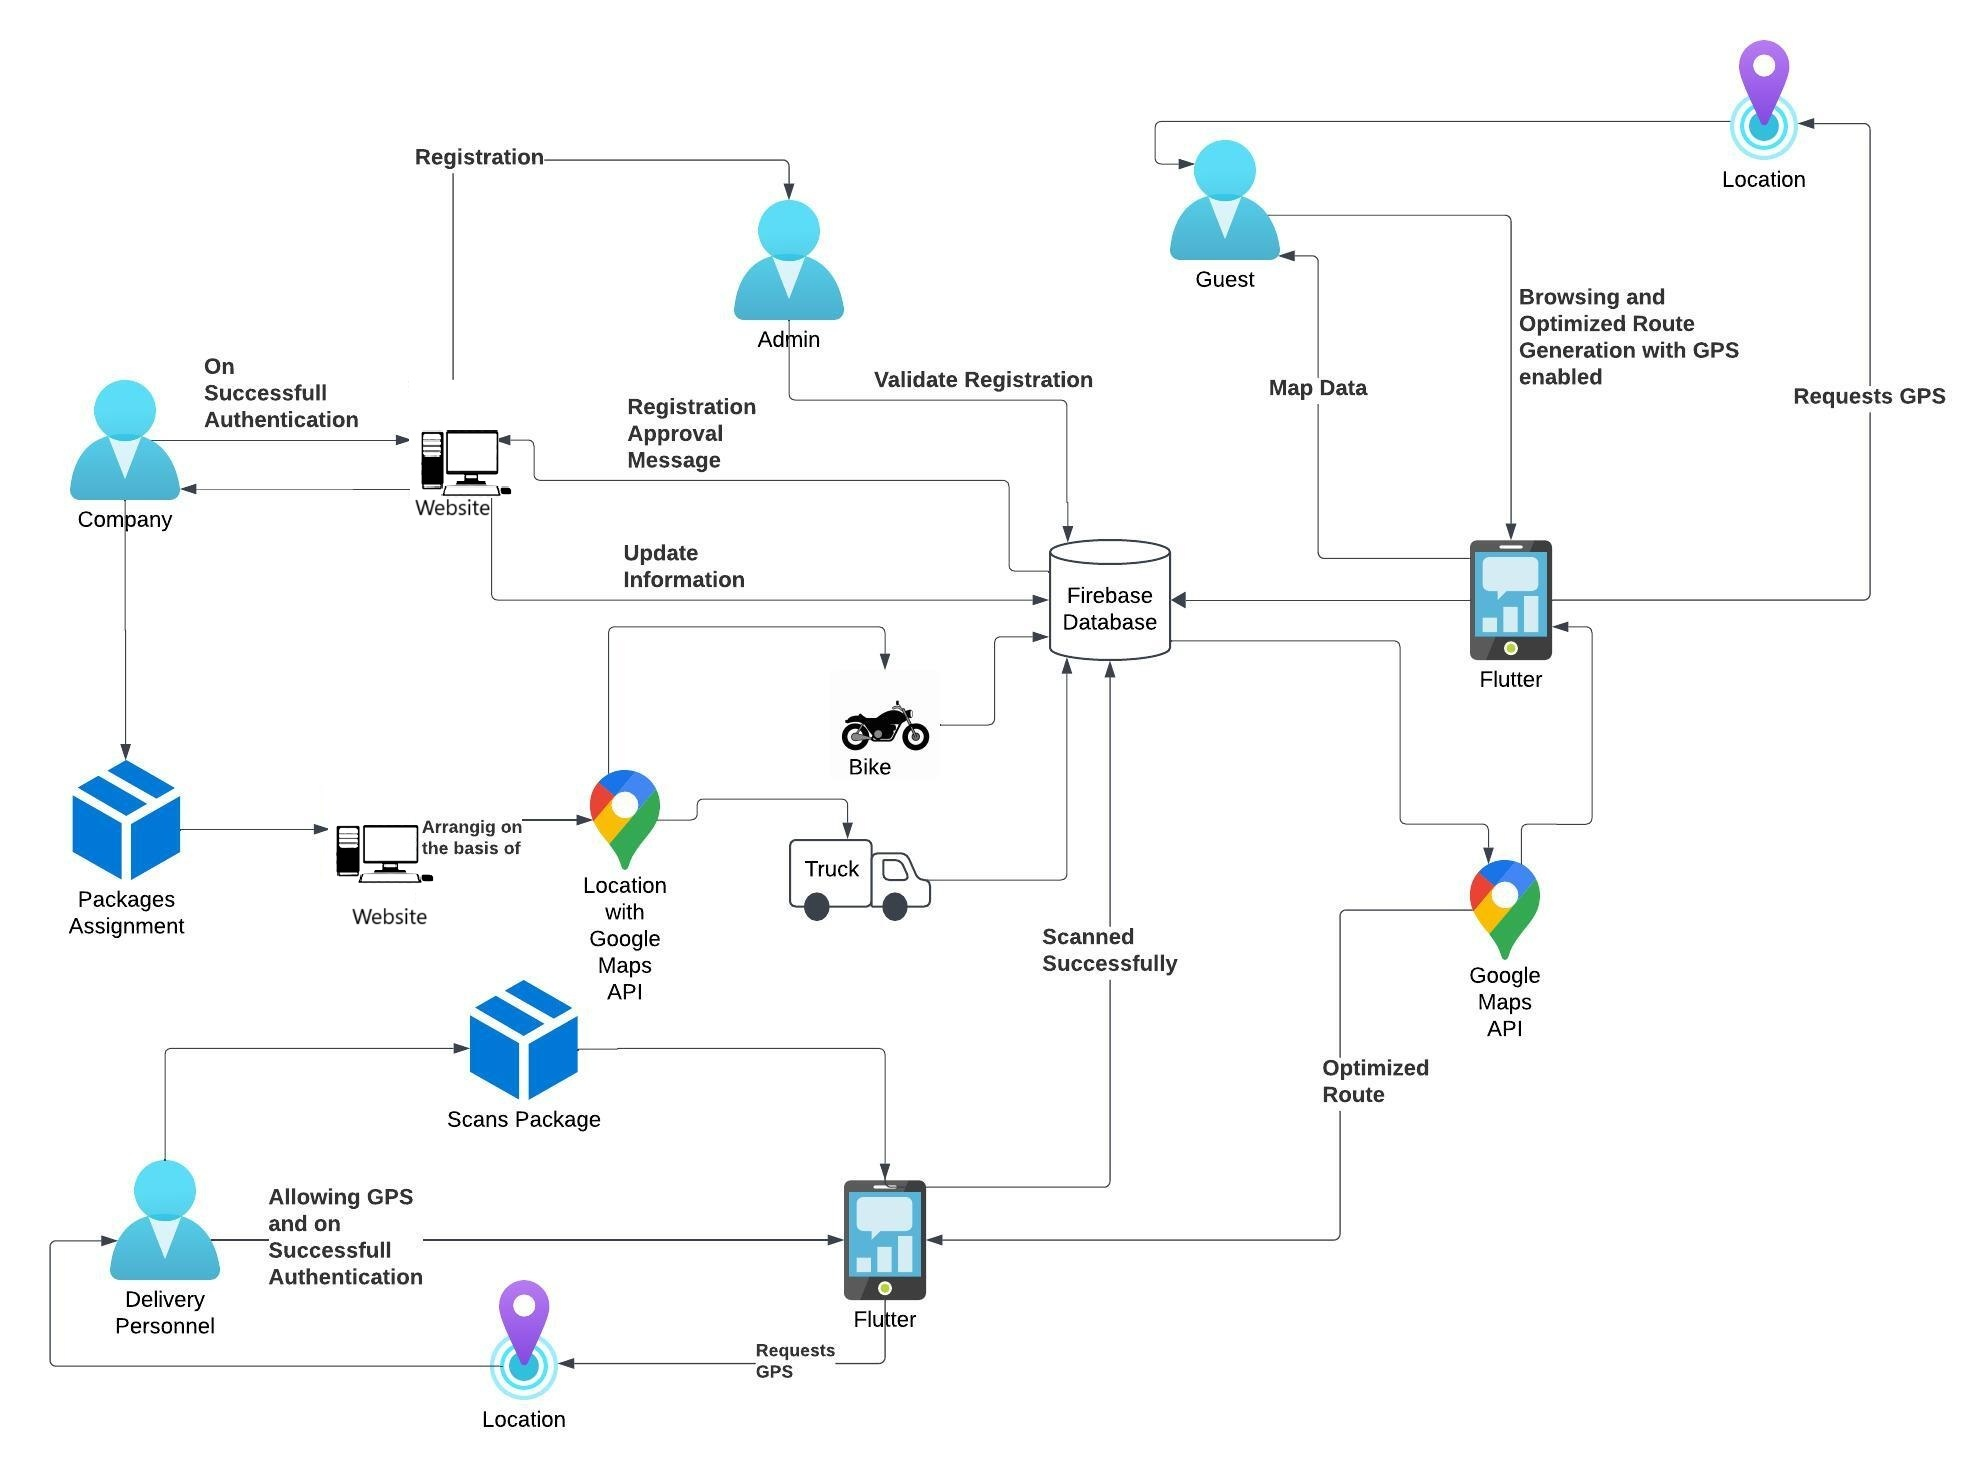
\includegraphics[scale=0.5]{System Architecture.jpeg}
    \caption{System Architecture Diagram}
    \label{fig:system_architecture}
\end{figure}
\newpage
\subsection{Entity-Relationship (ER) Diagram}
The ER Diagram for the FastTrack represents the database structure, showing entities, their attributes and relationships. The main entities are Company, Delivery Personnel, Admin and Package. Company registers on the platform and manages delivery personnel. Delivery Personnel are assigned packages and follow optimized routes for delivery.
Admin verifies company registrations and grants login credentials. Package is linked to a company and assigned to delivery personnel for delivery.
\begin{figure}[H]  % Use [H] to force the position
\centering
    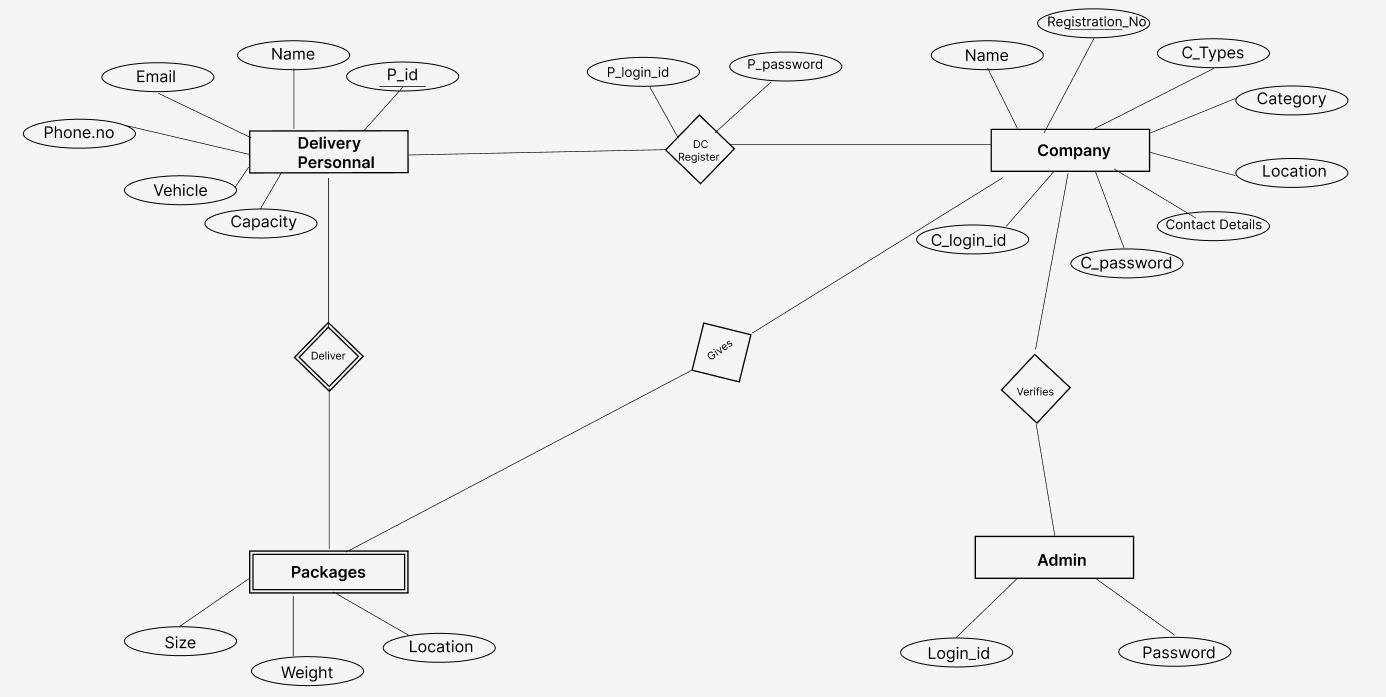
\includegraphics[scale=0.3]{ERdiagram2.jpg}
    \caption{ER Diagram}
    \label{fig:er_diagram2}
\end{figure}
\subsection{Algorithm Modules}
FastTrack incorporates the following algorithm modules:
\begin{itemize}
    \item Authentication Algorithm
    \item Company Registration Algorithm
    \item Update Information Algorithm
    \item Validate Registration Algorithm
        \item Package Assignment Algorithm
    \item Scan Package Algorithm
    \item Retrieve Optimized Route After Scanning Packages Algorithm
    \item Route Optimization with Google Maps API Algorithm
\end{itemize}
\newpage
\section{Detailed Design}
\subsection{Authentication Algorithm}
\SetKwComment{Comment}{/* }{ */}

\begin{algorithm}[hbt!]
\caption{Delivery Personnel or Company or Admin Authentication Algorithm}
\SetKwInOut{Input}{Input}
\SetKwInOut{Output}{Output}
\Input{\textnormal{LoginID and Password}}
\Output{\textnormal{Authentication status (Success/Failure message with token if successful)}}
\textnormal{Input the LoginID and Password from the user.}\\
\textnormal{Search for the LoginID in the user database.}\\
\If{the user with the LoginID is found}{
Validate the Password.\\
\If{the Password matches}{
Generate an Authentication Token.\\
Grant access.\\
Display "Authentication Successful".\\
}
\Else{
Display "Invalid Password,Try Again!".
}
}
\Else{
Display "User Not Found". 
}
\end{algorithm}
\subsection{Company Registration}
\begin{algorithm}[H]
\caption{Company Registration Algorithm}
\SetKwInOut{Input}{Input}
\SetKwInOut{Output}{Output}
\Input{Company Name, Registration Number, Type of Company, Business Category, Address, Contact Details, and Verification Documents}
\Output{Application Number and Validation Status}


Input Company Name, Registration Number, Type of Company, Business Category, Address and Contact Details.\\
Check if the registration number matches the official format using a regular expression.\\
\If{valid}{
    Check if contact details are valid.\\
    \If{valid}{
    Input Certificate of Incorporation, PAN Card and Proof of Address Documents.\\
    \If{Documents uploaded is NULL}{
    Display "Please upload the required documents".
    }
    \Else{
    Generate an application tracking number.\\
    Display "Validation Status: Pending Approval".
    }
    }
    \Else{Display "Invalid Contact Details".}
}
\Else{Display "Invalid Registration Number".}
\end{algorithm}
\subsection{Update Information Algorithm}
\begin{algorithm}[H]
\caption{Update Information}
\SetKwInOut{Input}{Input}
\SetKwInOut{Output}{Output}
\Input{
\textnormal{User Role: Admin, Company or Delivery Personnel \\Update options: Address, Contact Information, Business Category}
}
\Output{ 
    \textnormal{Update Status (Success or Failure)}\\
}
Input User Role: Admin, Company or Delivery Personnel.
\\
Verify User Login using Algorithm 1.\\
Capture the fields the user wants to update.\\
Access the corresponding database table.\\
Update the relevant fields with the new details.\\
\If{the database update fails}
{
Display "Error updating information. Please try again later".\\
Set Update Status as "Failure".\\
\Else{
Display "Information updated successfully".\\
Set Update Status as "Success".}
}
\end{algorithm}
\subsection{Validate Registration Algorithm}
\begin{algorithm}
\caption{Validate Registration}
\SetKwInOut{Input}{Input}
\SetKwInOut{Output}{Output}
\Input{
\textnormal{Certificate of Incooperation, PAN Number and Proof of Address}
}
\Output{Validation status (Valid/Invalid)
}

Input Certificate of Incooperation, PAN Number and Proof of Address.\\
Ensure the Certificate of Incorporation is uploaded.\\
Verify that the PAN Card matches the company name format.\\
Check if the Proof of Address is valid.\\
\If{All validation is done}{
set Validation Status as "Valid".\\
sent LoginID and temporary password to the company's email address.\\
\Else{
set Validation Status as "Invalid".\\
sent a message "Validation Failed due to incorrect document submission" to the company's email address.\\
}
}
\end{algorithm}
\subsection{Package Assignment Algorithm}
\small 
\begin{algorithm}
\caption{Package Assignment}
\SetKwInOut{Input}{Input}
\SetKwInOut{Output}{Output}
\Input{
    \textnormal{An Excel sheet, which includes package ID, location, weight, size, and date.}\\
    	\textnormal{Average weight and size capacity of the vehicles used for delivery.}\\
        \textnormal{Warehouse location}
}
\Output{
    \textnormal{Table with assigned Employee ID, Package ID, Location, and Date}
}
Dividing packages into four quadrants based on their delivery location:
Quadrants = {"NE": [], "NW": [], "SW": [], "SE": []}\\

Categorize packages by Algorithm 6\\

Categorize packages by vehicles based on, bikes can carry packages labeled lvs, ls, lm, ms, and mm, while trucks can carry packages labeled ll, ml, hs, hm, hl, hym, and hyl.\\

Calculate the total weight and size for both bikes and trucks, add any remaining weight and size to the current weighted size during the calculation.\\

Use Algorithm 7 to find number of employees for bike and truck.\\

Input Number of Employees for bikes and trucks\\

Assign packages to bike employees by Algorithm 8\\

\If{Total weight of Bpackage_remaining $\geq $125kg
}{Average weight of truck = 125kg\\
Average size of truck = 500cm³\\
\[
m = \frac{\text{Total weight of Bpackage remaining}}{\text{Average weight of truck}}
\]

\[
n = \frac{\text{Total size of Bpackage remaining}}{\text{Average size of truck}}
\]

\[
\text{Truck\_employee2} = \max(m, n)
\]

\[
\text{Total\_Truck\_employee} = \text{Truck\_employee} + \text{Truck\_employee2}
\]}

Assign packages to truck employees by Algorithm 9\\
\end{algorithm}

\begin{algorithm}
\caption{Categorize Packages}
\SetKwInOut{Input}{Input}
\SetKwInOut{Output}{Output}
\Input{
\textnormal{package ID, location, weight and size}
}
\Output{ 
    \textnormal{Categorized package list 
}
}
\ForEach{weight in packages}{
Extract weight $w$ and size $s$ from $p$\;
 \If{$w < 2$ \textbf{and} $s <$ verysmall}{
        Assign $p$ to category \texttt{lvs}\;
    }
    \ElseIf{$w < 2$ \textbf{and} $s <$ small}{
        Assign $p$ to category \texttt{ls}\;
    }
    \ElseIf{$w < 2$ \textbf{and} $s <$ medium}{
        Assign $p$ to category \texttt{lm}\;
    }
    \ElseIf{$2 < w < 5$ \textbf{and} $s <$ small}{
        Assign $p$ to category \texttt{ms}\;
    }
    \ElseIf{$2 < w < 5$ \textbf{and} $s <$ medium}{
        Assign $p$ to category \texttt{mm}\;
    }
    \ElseIf{$w < 2$ \textbf{and} $s <$ large}{
        Assign $p$ to category \texttt{ll}\;
    }
    \ElseIf{$2 < w < 5$ \textbf{and} $s <$ large}{
        Assign $p$ to category \texttt{ml}\;
    }
    \ElseIf{$5 < w < 15$ \textbf{and} $s <$ small}{
        Assign $p$ to category \texttt{hs}\;
    }
    \ElseIf{$5 < w < 15$ \textbf{and} $s <$ medium}{
        Assign $p$ to category \texttt{hm}\;
    }
    \ElseIf{$5 < w < 15$ \textbf{and} $s <$ large}{
        Assign $p$ to category \texttt{hl}\;
    }
    \ElseIf{$w > 15$ \textbf{and} $s <$ medium}{
        Assign $p$ to category \texttt{hym}\;
    }
    \ElseIf{$w > 15$ \textbf{and} $s <$ large}{
        Assign $p$ to category \texttt{hyl}\;
    }
}
\end{algorithm}

\begin{algorithm}
\caption{Assigning Algorithm for Bike and Truck Employees}
\SetKwInOut{Input}{Input}
\SetKwInOut{Output}{Output}
\Input{
    \textnormal{Packages with weight, size, and location.}\\
    \textnormal{Vehicle capacity (average weight and size).}
}
\Output{
    \textnormal{Assigned employees and optimized routes.}
}

\While{Total\_Weight\_Vehicle $\neq$ 0}{ 
    
    \While{\textnormal{Quadrants changing}}{
        
        \While{\textnormal{Each employee is processing}}{ 
            
            \While{Average\_Weight $\neq$ 0 \textbf{and} Average\_Size $\neq$ 0}{
                Assign package\;
                Update Average\_Weight, Average\_Size\;
                
                \If{\textnormal{Remaining space but no suitable package}}{
                    
                    \If{Average\_Weight $>$ 4}{
                        Move to next quadrant (i → i+1)\;
                        Assign available package\;
                    }
                    
                    \If{Average\_Weight $<$ 4}{
                        Move to next quadrant (i → i+1)\;
                        \If{Average\_Weight == Package\_Weight \textbf{and} Average\_Size == Package\_Size}{
                            Perform route optimization\;
                            Compute shortest path (Dijkstra’s algorithm)\;
                            \If{Distance $<$ MAX\_DISTANCE}{
                                Assign package and update weight/size\;
                            }
                        }
                    }
                }
            }
        }
    }
}
\end{algorithm}
\begin{algorithm}
\caption{Assigning Packages to Bike Employees}
\SetKwInOut{Input}{Input}
\SetKwInOut{Output}{Output}
\Input{
    \textnormal{Bike employees count, available employees, and assigned packages.}
}
\Output{
    \textnormal{Updated package assignment and remaining packages.}
}

\If{Bike\_employees == Available\_employeesB}{
    Assign packages using \texttt{assigned\_packages[]} from Algorithm 7\;
}

\If{Bike\_employees > Available\_employeesB}{
    Assign packages to available employees\;
    Store remaining packages in \texttt{Bpackages\_remaining}\;
    Prioritize remaining packages for the next working day\;
}

Calculate total weight and size of \texttt{Bpackage\_remaining}\;

\end{algorithm}
\begin{algorithm}
\caption{Truck Employee Allocation and Package Assignment}
\SetKwInOut{Input}{Input}
\SetKwInOut{Output}{Output}
\Input{
    \textnormal{Total Truck Employees required (\texttt{Total\_Truck\_employees})}\\
    \textnormal{Available Truck Employees (\texttt{Available\_EmployeesT})}
}
\Output{
    \textnormal{Assigned employees and remaining packages}
}

\If{Truck\_employees == Available\_EmployeesT}{
    Assign packages to employees\;
    \texttt{Bpackage\_remaining} remains unchanged and is prioritized for the next working day\;
}

\If{Truck\_employees > Available\_EmployeesT}{
    Assign packages to \texttt{Available\_EmployeesT}\;
    Store remaining packages in \texttt{Tpackage\_remaining} and prioritize for the next working day\;
    \texttt{Bpackage\_remaining} remains unchanged and prioritized for the next working day\;
}

\If{Total\_Truck\_employees == Available\_EmployeesT}{
    \If{Truck\_employees == Available\_EmployeesT - Truck\_employee2}{
        Assign packages to employees\;
        Assign \texttt{Bpackage\_remaining} to employees\;
    }
}

\If{Total\_Truck\_employees > Available\_EmployeesT \textbf{and} Truck\_employees < Available\_EmployeesT}{
    \texttt{Emp} $\gets$ Available\_EmployeesT - Truck\_employees\;
    
    \If{Truck\_employees == Available\_EmployeesT - Emp}{
        Assign packages to employees\;
    }

    \If{Truck\_employee2 > Emp}{
        Assign \texttt{Bpackage\_remaining} to \texttt{Emp}\;
        Store remaining packages in \texttt{Bpackages\_remaining} and prioritize for the next working day\;
    }
}

\end{algorithm}
\subsection{Scan Package}
\begin{algorithm}[H]
\caption{Scan Package}
\SetKwInOut{Input}{Input}
\SetKwInOut{Output}{Output}
\Input{
\textnormal{Package ID (from the scanned QR code)}
}
\Output{ 
    \textnormal{Scanning Status (Success or Failure) 
}
}
Verify Login using Algorithm 1.\\
Extract the Package ID from the scanned data.\\
Check if the Package ID exists in the system's database.\\
\If{not found}
{
Display "Invalid Package ID. Please scan a valid package".\\
Set Scanning Status as "Failure".\\
}
\Else{
Update the package record in the database\\
Set Scanning Status as "Success."\\
Display "Package successfully scanned and assigned for delivery."\\
}
\end{algorithm}
\subsection{Retrieve efficient Route After Scanning Packages}
\begin{algorithm}[H]
\caption{Retrieve efficient Route After Scanning Packages Algorithm}
\SetKwInOut{Input}{Input}
\SetKwInOut{Output}{Output}
\Input{
\textnormal{Delivery Personnel ID\\
Scanned Package IDs}
}
\Output{ 
    \textnormal{
    Route Map (Efficient delivery route) or Error Message
}\\
}
Verify Login using Algorithm 1.\\
Ensure all assigned Package IDs are scanned.\\
\If{not all assigned packages are scanned}
{Display "Not all assigned packages are scanned."}
\Else{
Retrieve the efficient Route generated by the company for this specific set of packages.\\
\If{no route exists}
{Display "Optimized route not available."}

\Else{
Display the efficient Route Map on the delivery personnel’s interface.
}}
\end{algorithm}
\newpage
\subsection{Route Optimization with Google Maps API Algorithm}
\begin{algorithm}
\caption{Route Optimization with Google Maps API}
\SetKwInOut{Input}{Input}
\SetKwInOut{Output}{Output}
\Input{
\textnormal{Delivery locations (latitude, longitude)}
}
\Output{ 
    \textnormal{Optimized delivery route and total distance}\\
}
Input Delivery Locations as latitude and longitude pairs.\\
Send the locations to Google Maps Distance Matrix API.\\
Receive pairwise distances and travel times between all locations.\\
Set the first location as the starting point.\\
Initialize an empty route list and add the starting location.\\
Optimize Route Using Greedy Algorithm.\\
\While{there are unvisited locations}
{
    Find the nearest unvisited location using the distance matrix\\
    Add the nearest location to $route$\\
    Mark the location as visited\\
}
Add the starting location to the end of the route to complete the cycle.\\
For calculating the total distance, sum the distances between consecutive locations in the route using the distance matrix.\\
Display the optimized route sequence and integrate with Google Maps for visualization.\\
Print the total distance.\\
\end{algorithm}
\section{Summary}
Chapter 3 of the software development life cycle (SDLC) delves into the design phase, transitioning
from problem identification to solution planning. It encompasses two key stages: System Design and
Detailed Design. The System Design phase defines key system components, interactions and data
flow using DFDs, use case diagrams, system architecture and ER diagrams. The Detailed Design
phase elaborates on essential algorithms, including authentication, company registration, update
information, validate registration, package assignment, scan package, retrieving efficient route and
route optimization.